\subsubsection{Opis przypadków użycia - pracownik}

Opis przypadków użycia dotyczących funkcjonalności związanych z zarządzaniem
pracownikami:

\begin{figure}[h!]
    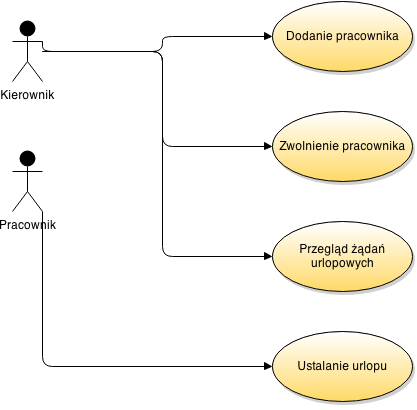
\includegraphics[width=\textwidth,
    height=0.5\textheight]{graphics/UseCase/Pracownik/UseCaseDiagram.png}
  \caption{Diagram przypadków użycia związanych z procesowaniem danych
  pracowników}
\end{figure}

\begin{enumerate}
  
  \item Dodawanie pracownika \\
  \begin{tabularx}{\linewidth}{ c X }
  Aktor: & Kierownik \\
  Opis: & Możliwość zatrudnienia nowego pracownika.\\
  \end{tabularx}
   \begin{enumerate}
    \item Kierownik uruchamia stronę internetową panelu zarządzania sklepem
    i~wybiera opcję rejestracji.
    \item Kierownik wprowadza dane osobowe zatrudnianego pracownika.
    \item System sprawdza wstawione dane (czy istnieje już zarejestrowany
    w~systemie użytkownik, czy istnieje podany adres e-mail itp.)
    \item System wysyła na adres e-mail pracownika podany przez~kierownika
    wiadomość powitalną wraz z~linkiem umożliwiającym aktywowanie konta oraz
    ustalenie hasła.
    \item W ciągu określonego, zdefiniowanego czasu pracownik odwiedza stronę
    o~adresie przesłanym w~wiadomości powitalnej i ustala hasło dla konta.
  \end{enumerate}

  \item Zwolnienie pracownika \\
  \begin{tabularx}{\linewidth}{ c X }
  Aktor: & Kierownik \\
  Opis: & Możliwość zwolnienia pracownika.\\
  \end{tabularx}
   \begin{enumerate}
    \item Kierownik uruchamia stronę internetową panelu zarządzania sklepem i~wybiera panel zarządzania pracownikami.
    \item Kierownik wyszukuje odpowiedniego pracownika.
    \item System wyświetla pracowników spełniających zadane kryteria wyszukiwania.
    \item Kierownik wybiera odpowiedniego pracownika.
    \item Kierownik wybiera opcję ,,Zwolnij''.
    \item System wyświetla formularz zwolnienia.
    \item Kierownik wypełnia formualrz podając przyczynę zwolnienia oraz datę od której pracownik ma być zwolniony.
    \item System sprawdza poprawność formualrza (np. czy można zwolnić pracownika w terminie wskazanym przez kierownika).
    \item W przypadku błędów system wyświetla odpowiedni komunikat, a kierownik poprawia dane w formularzu.
    \item System wyświetla prośbę o potwierdzenie operacji (dane pracownika oraz pytanie czy na pewno intencją kierownika
    było jego zwolnienie).
    \item Pracownik zatwierdza operację.
    \item System zapisuje informację o zwolnieniu pracownika.
    \item W momencie zaczęcia obowiązywania zwolnienia, system archiwizuje dane pracownika i~usuwa
    go~z~grupy zatrudnionych osób.
  \end{enumerate}
  
  \item Ustalanie urlopu \\
  \begin{tabularx}{\linewidth}{ c X }
  Aktor: & Pracownik \\
  Opis: & Możliwość zgłoszenia prośby o urlop.\\
  \end{tabularx}
  \begin{enumerate}
    \item Pracownik uruchamia aplikację internetową sklepu i loguje się do systemu.
    \item Pracownik wybiera panel urlopów.
    \item System informuje pracownika o ilości dni urlopowych pozostałych do wykorzystania.
    \item Pracownik dodaje do kalendarza firmowego nowe żądanie urlopu.
    \item Pracownik uzupełnia dane dotyczące czasu przebywania na urlopie (datę początkową oraz datę końcową).
    \item System sprawdza, czy żądanie pracownika jest poprawne (np. czy pracownik może wziąć tak długi urlop).
    Jeśli nie, pracownik jest informowany o przyczynie błędu i musi ponownie wypełnić dane o urlopie.
    \item System zapisuje żądanie urlopu i informuje użytkownika o zmianie statusu żądania
    na~,,Oczekiwanie na odpowiedź kierownika''.
    \item Kierownik przegląda żądanie zgodnie ze scenariuszem ,,Przeglądanie żądań urlopowych''.
    \item Pracownik jest informowany o rozpatrzeniu żądania.
  \end{enumerate} 
  
  \item Przeglądanie żądań urlopowych \\
  \begin{tabularx}{\linewidth}{ c X }
  Aktor: & Kierownik \\
  Opis: & Możliwość przeglądania i rozpatrywania żądań urlopowych napływających od pracowników.\\
  \end{tabularx}
  \begin{enumerate}
    \item Kierownik loguje się do aplikacji internetowej systemu.
    \item Kierownik wybiera panel zarządzania pracownikami i przechodzi do sekcji ,,Urlopy''.
    \item System wyświetla kalendarz, w którym umieszczone są terminy urlopów.
    \item Kierownik ustawia odpowiednie filtry urlopów (np. wyświetlanie tylko nierozpatrzonych żądań).
    \item Kierownik wybiera jeden z urlopów i zmienia jego status.
    \item System sprawdza czy zmiana statusu jest poprawna (np. czy nie wystąpiła zmiana statusu z ,,Zrealizowany'' na ,,Odwołany'').
    \item W przypadku błędnej operacji system informuje o tym kierownika.
  \end{enumerate}

\end{enumerate}